\chapter{实验结果及分析}

\section{Auto Lab 测试合集}

四周 Lab 的 Auto Lab 测试合集如图\ref{fig:Autolabs}所示。我们按时,提前完成了每次的 AutoLab 测试。

\begin{figure}
    \centering
    \subfigure[Lab1 AutoLab 测试结果]{\label{fig:autolab}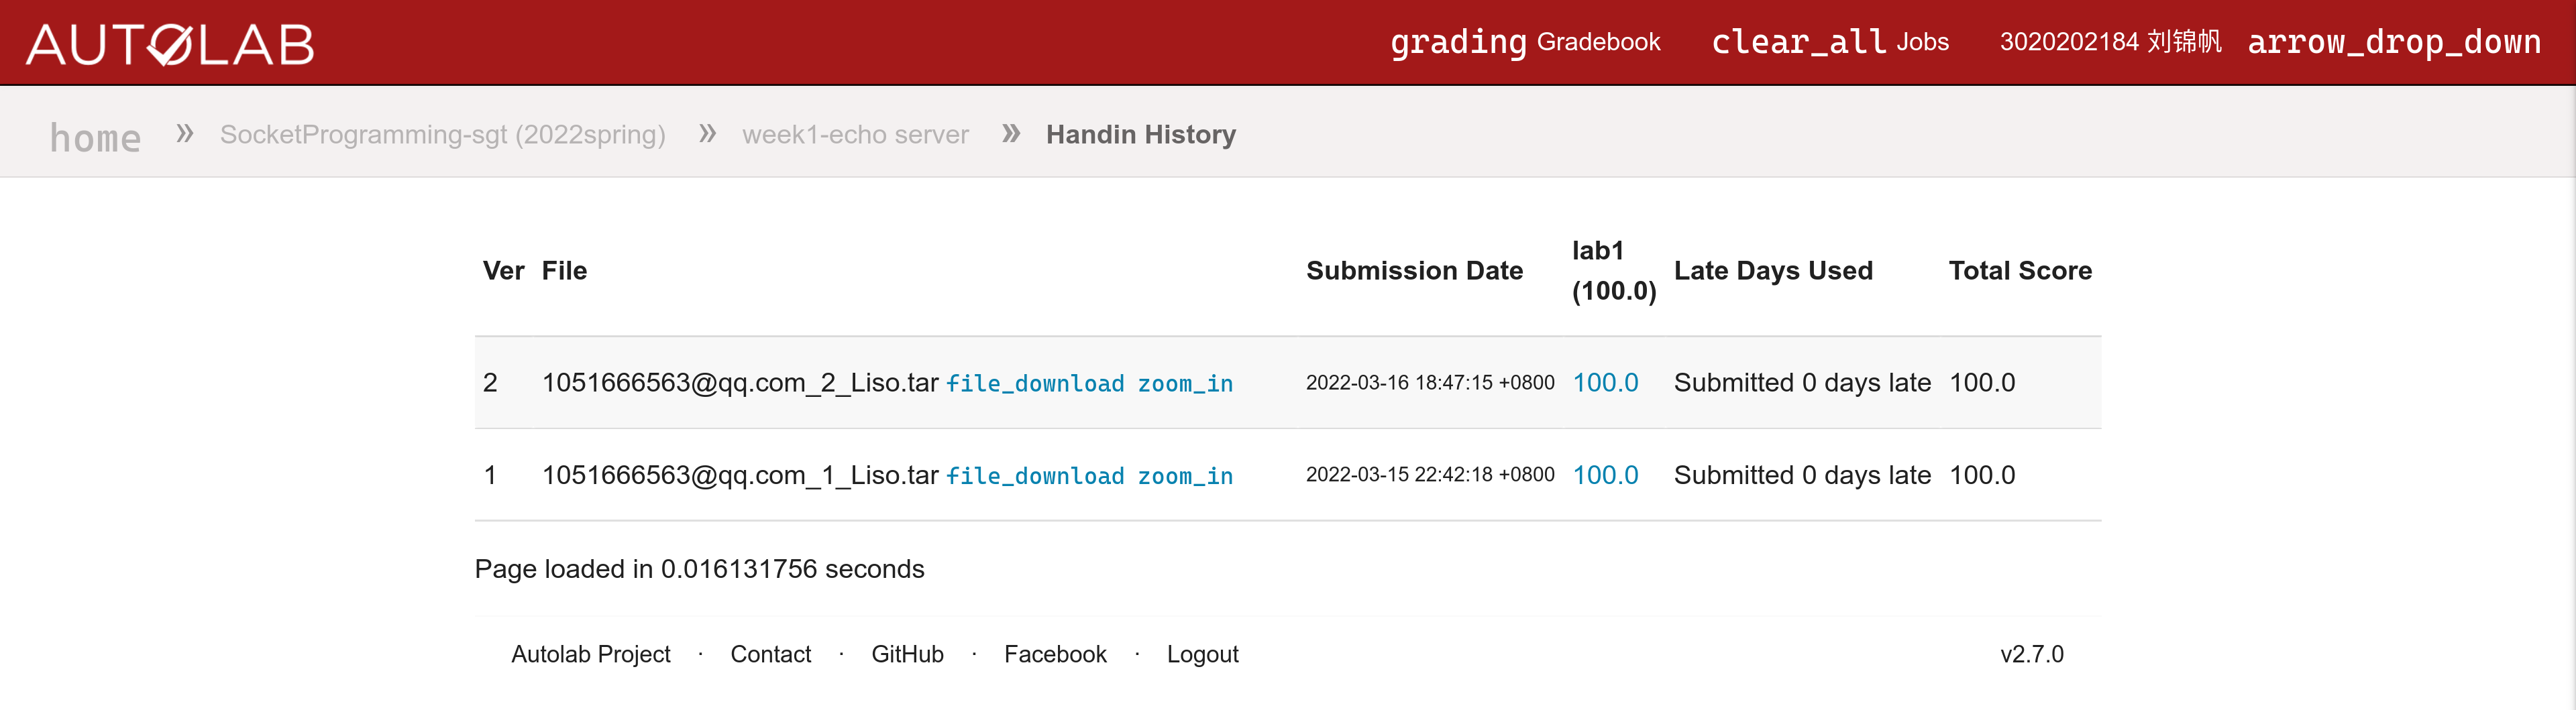
\includegraphics[width=5.5in]{autolab_uploaded.png}}
    \subfigure[Lab2 AutoLab 测试结果]{\label{fig:lab2autolab}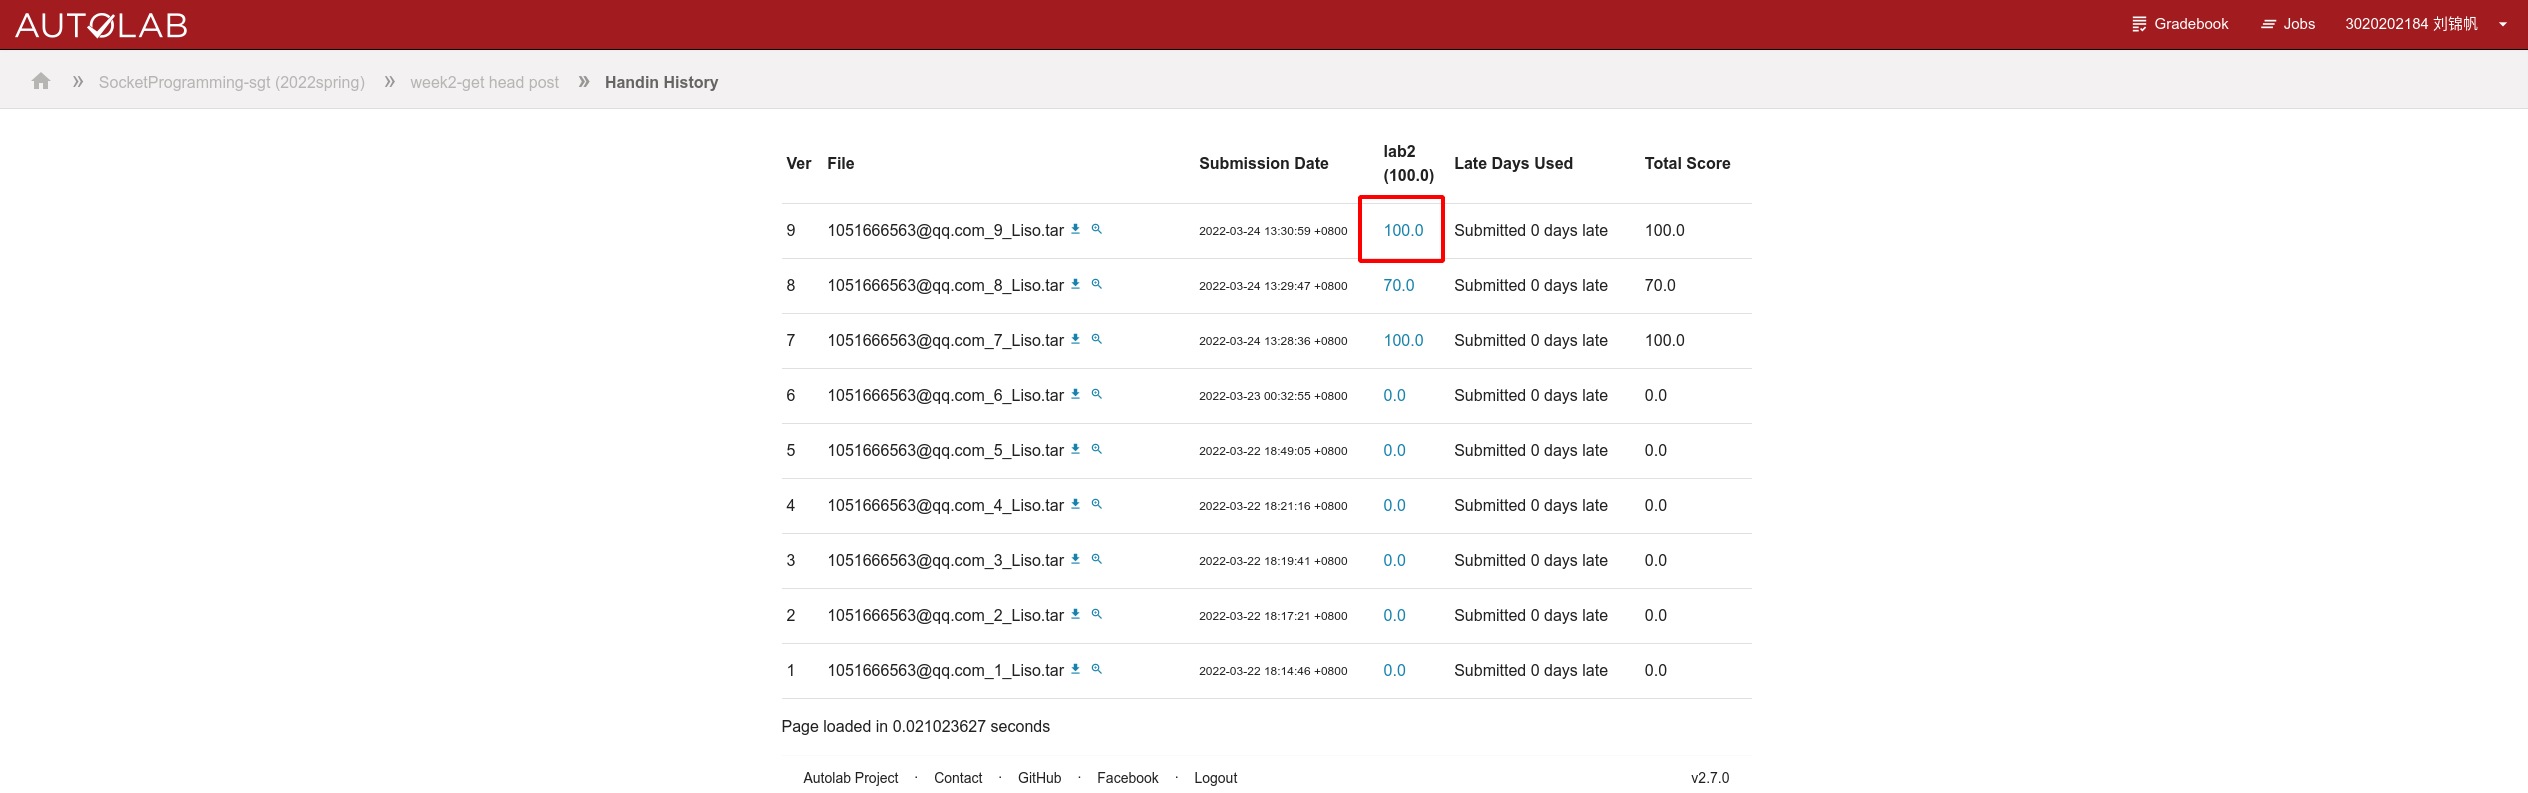
\includegraphics[width=5.5in]{autolab2.png}}
    \subfigure[Lab3 AutoLab 测试结果]{\label{fig:autolab3}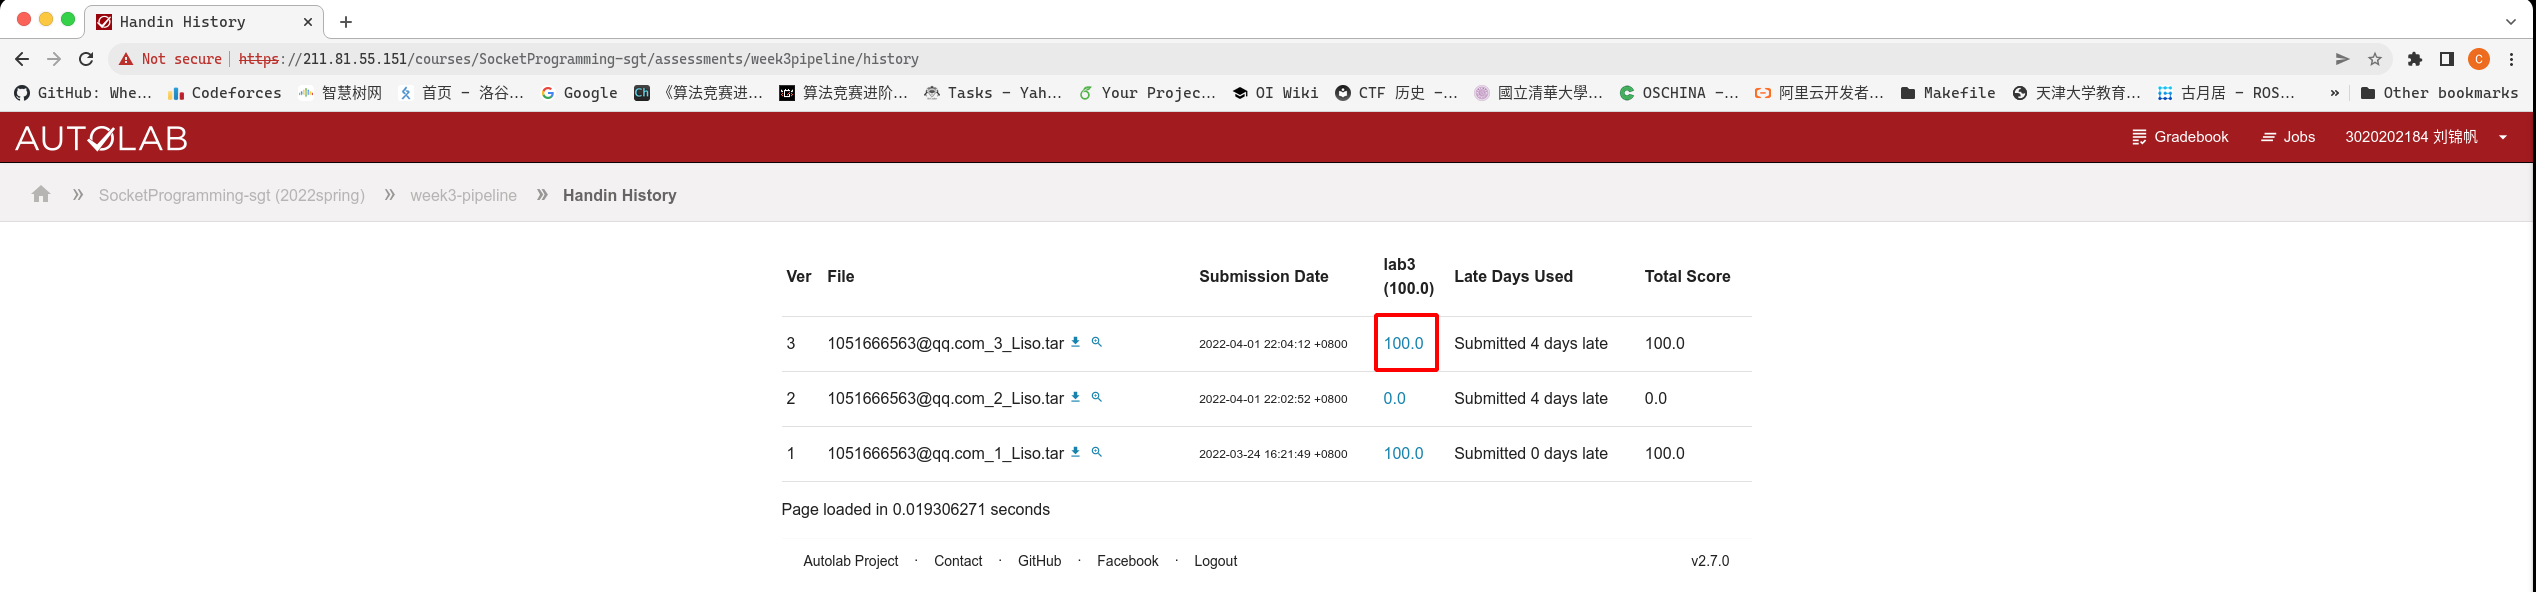
\includegraphics[width=5.5in]{autolab3.png}}
    \subfigure[Lab4 AutoLab 测试结果]{\label{fig:autolab4}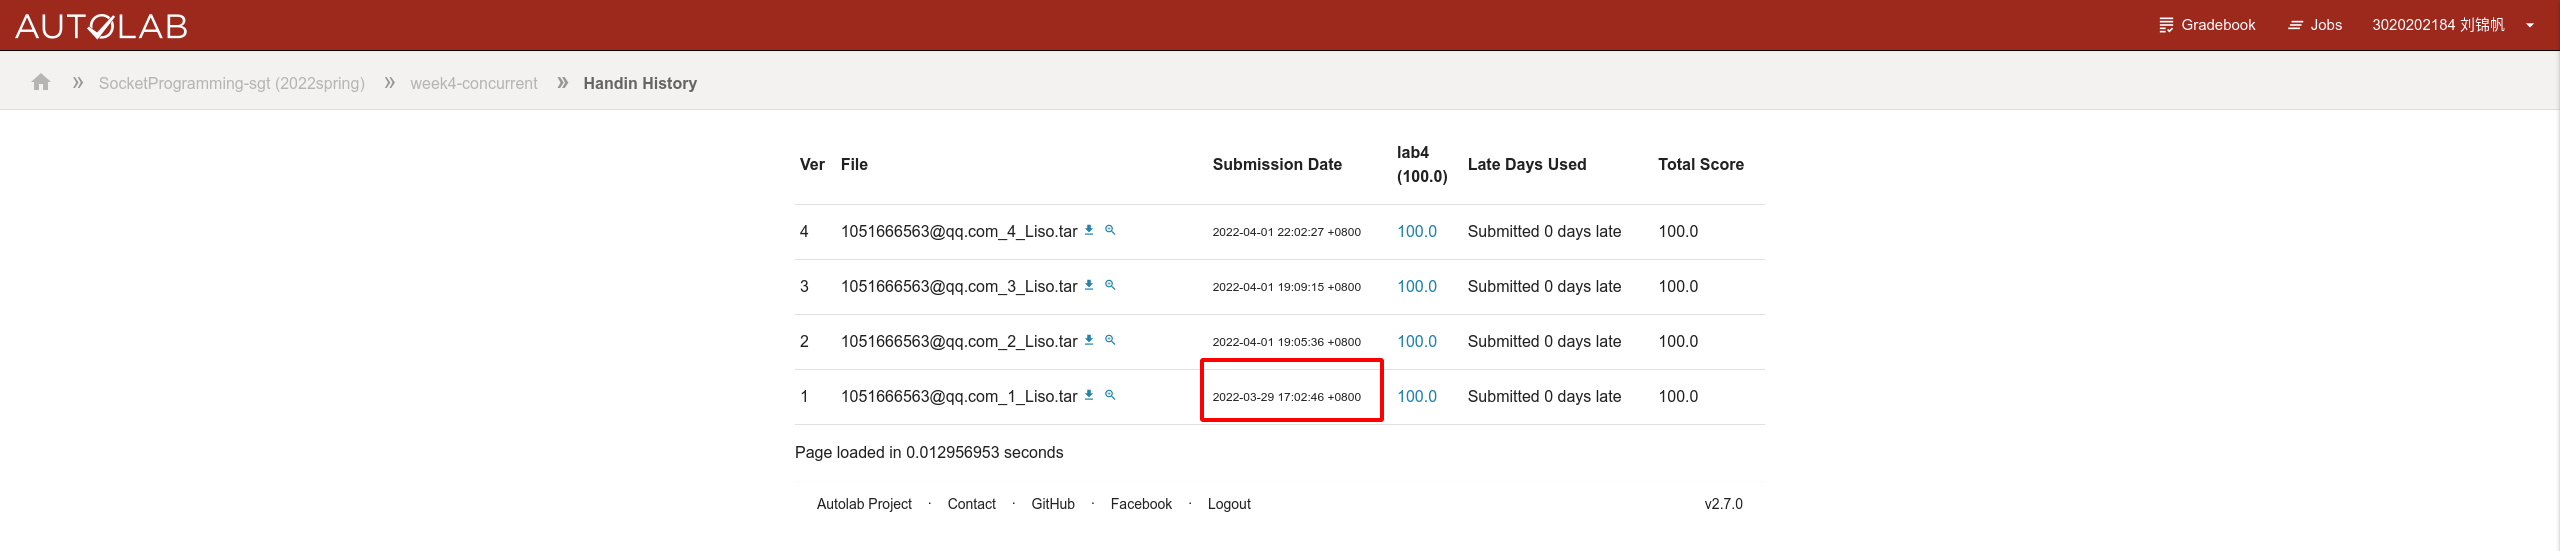
\includegraphics[width=5.6in]{autolab4.png}}
    \caption{AutoLab 测试合集}\label{fig:Autolabs}
\end{figure}

\section{第一周——实现简单的 echo web server}

在第一周中,我们主要对消息解析和 Echo Web Server 做了本地的测试。

\subsection{对消息的正确解析}

在 Makefile 中增加一项 test\_example 来批量测试 example,结果如图\ref{fig:maketestexample}所示。其中 Makefile 增加的脚本如下:

\begin{lstlisting}[language=C, name={Makefile: test example}]
test_example: example
@for f in $(shell ls samples); do \
	echo "=====Test file" $$f "========="; \
	./example samples/$$f | grep Segmentation --color ; \
	echo "---------------------------------------\n"; \
done
\end{lstlisting}

\subsubsection*{结果分析}

可以看到结果只在 error2, error3, error4 和 error5 四个情况下出现了 syntax error 的返回值,因为我们在 parser.y 增加了对测试样例中的 400 做了特殊处理,所以不会出现解析错误。且在 Makefile 中将 parse.c 原本的输出给屏蔽了,所以也不会有多余输出。

\subsection{echo web server}

实验操作如下:
\begin{enumerate}
    \item 在 echo\_client 中增加直接从文件中读取的支持;
    \item 先打开 echo\_server;
    \item 然后通过 echo\_client 发送一系列文件,查看 echo\_server 的结果。
\end{enumerate}

\subsubsection*{实验结果截图及分析}
实验结果如图\ref{fig:echo web server}所示。可以看到,在 head, get 和 post方法的实验中,我们实现了 echo 的效果。在 400 和 501 的输入中,我们实现了相应的返回消息。在输入文件不存在时,我们也得到了相应的正确返回,体现了我们程序的鲁棒性。

\begin{figure}[htbp!]
    \centering
    \subfigure[Head get and post actions]{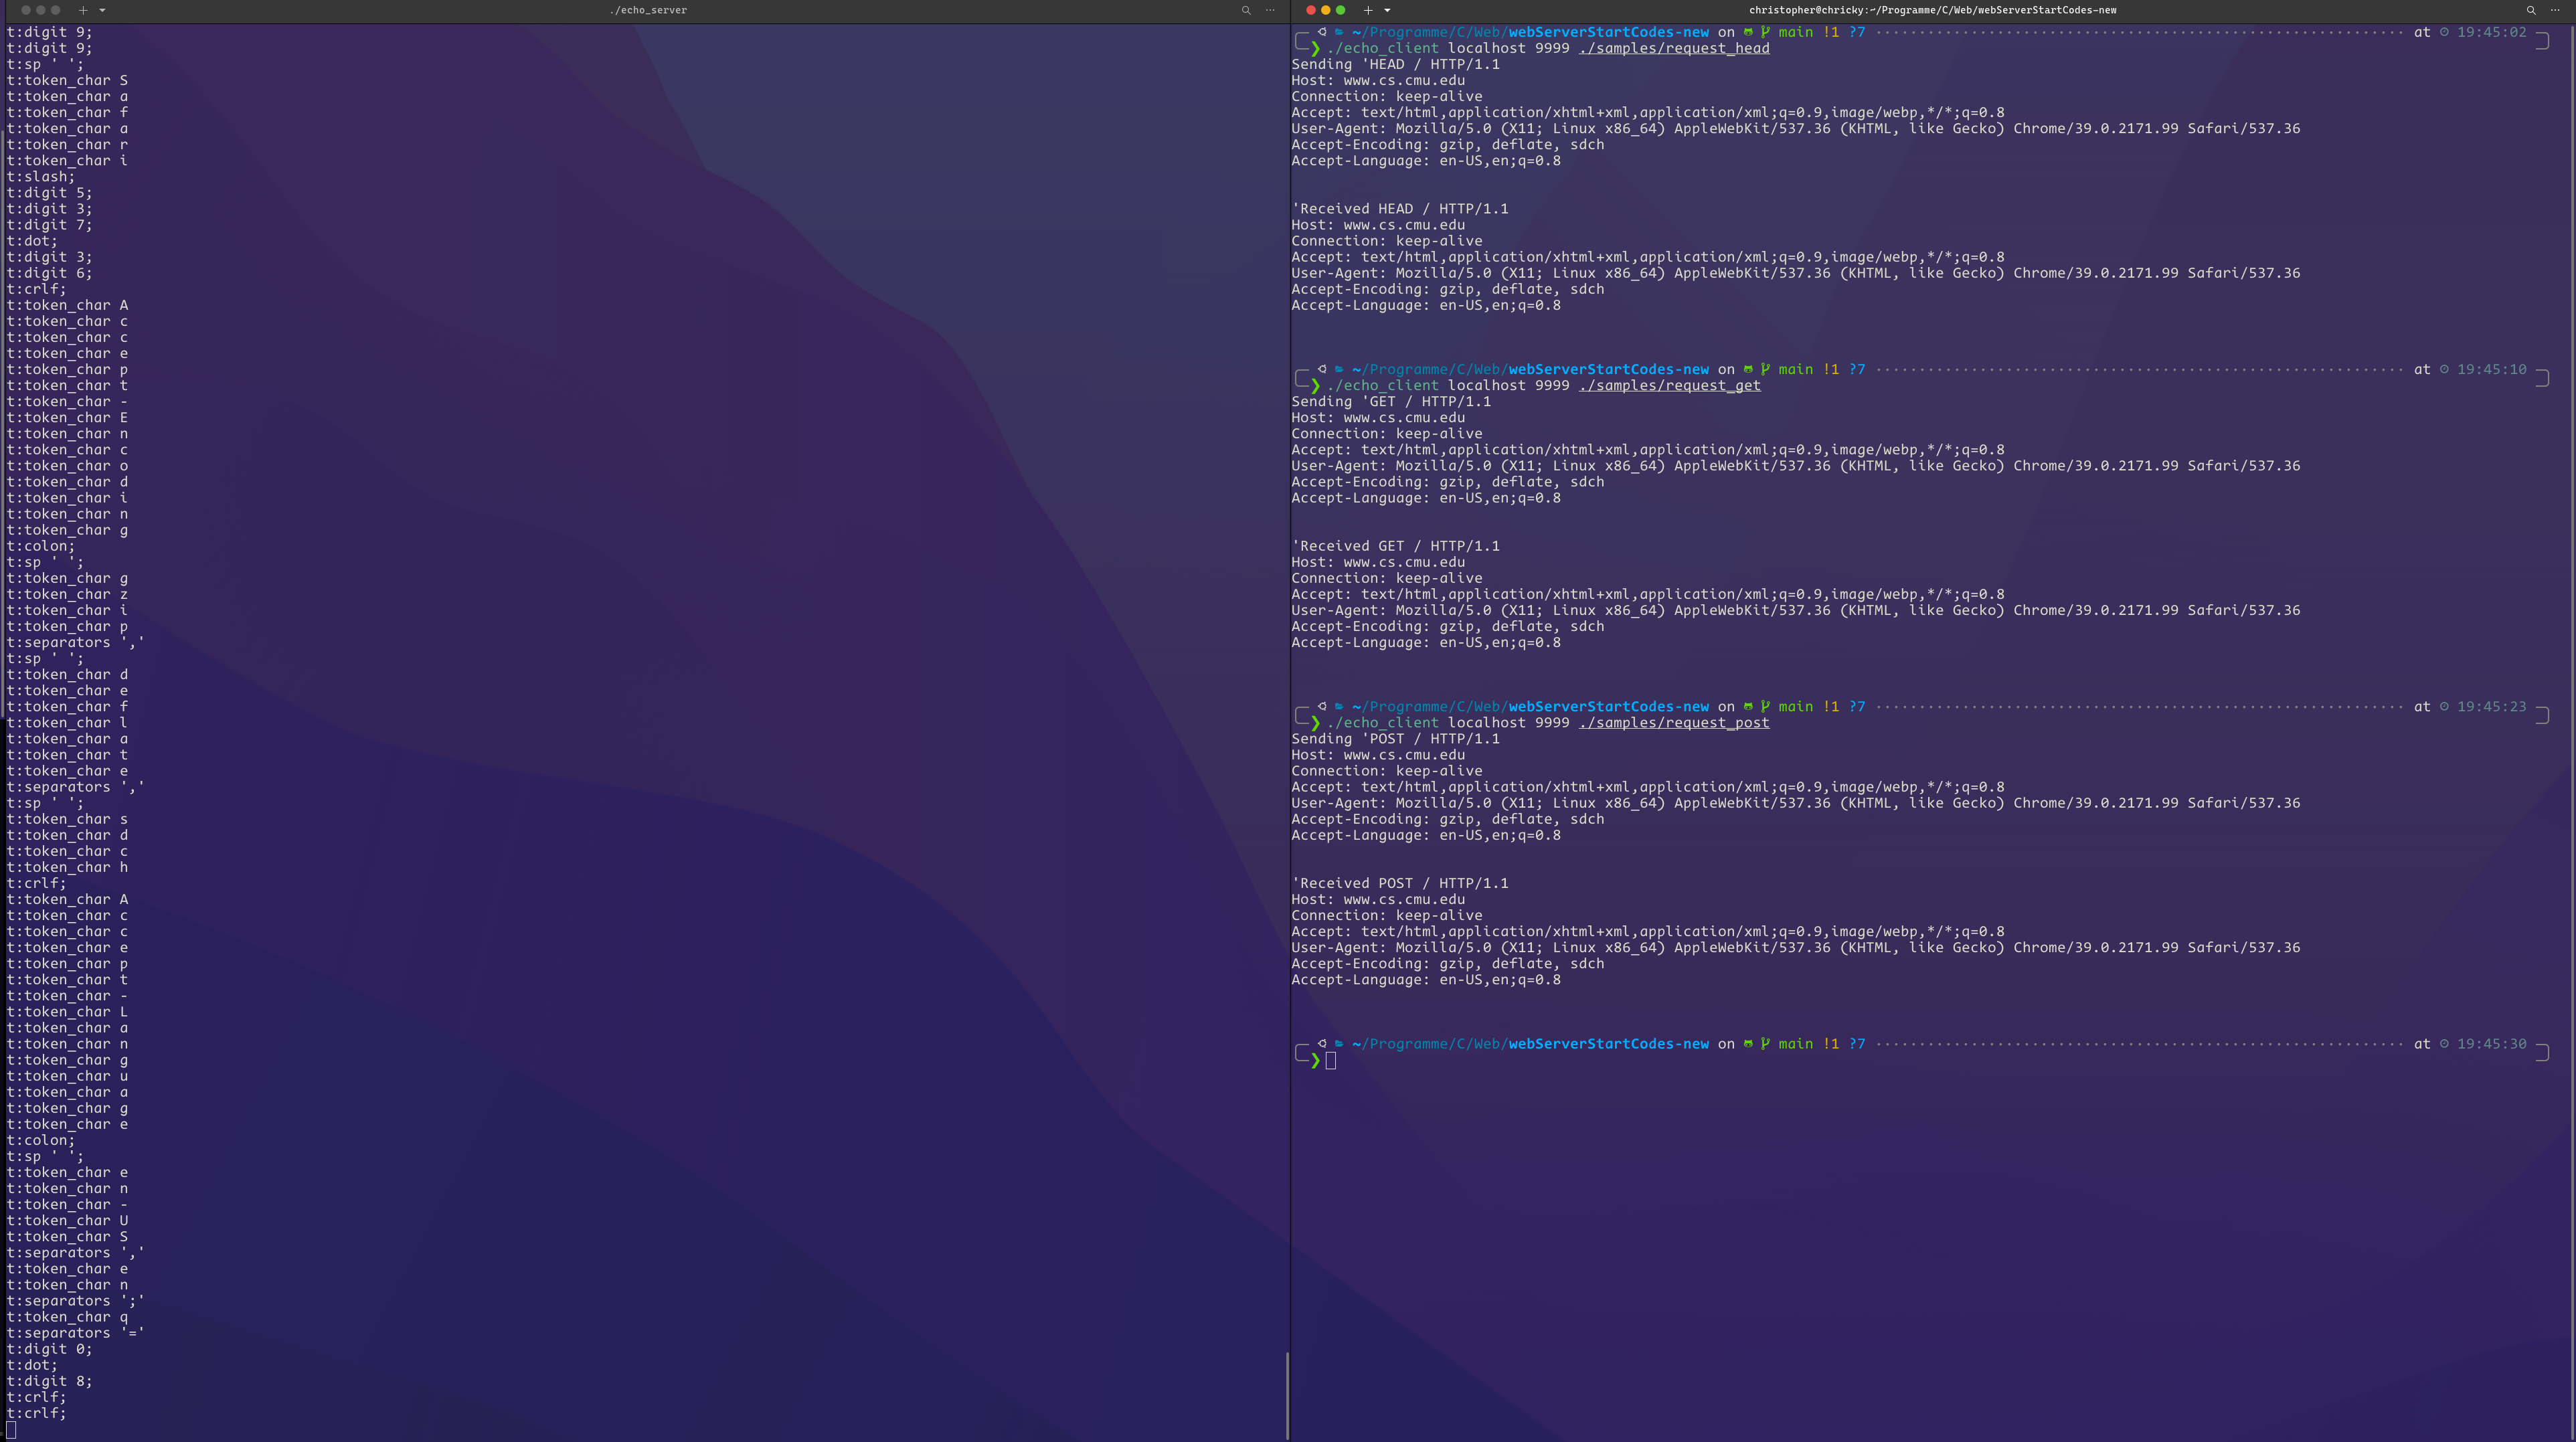
\includegraphics[width=2.5in]{head_get_post.png}}
    \subfigure[400 and 501]{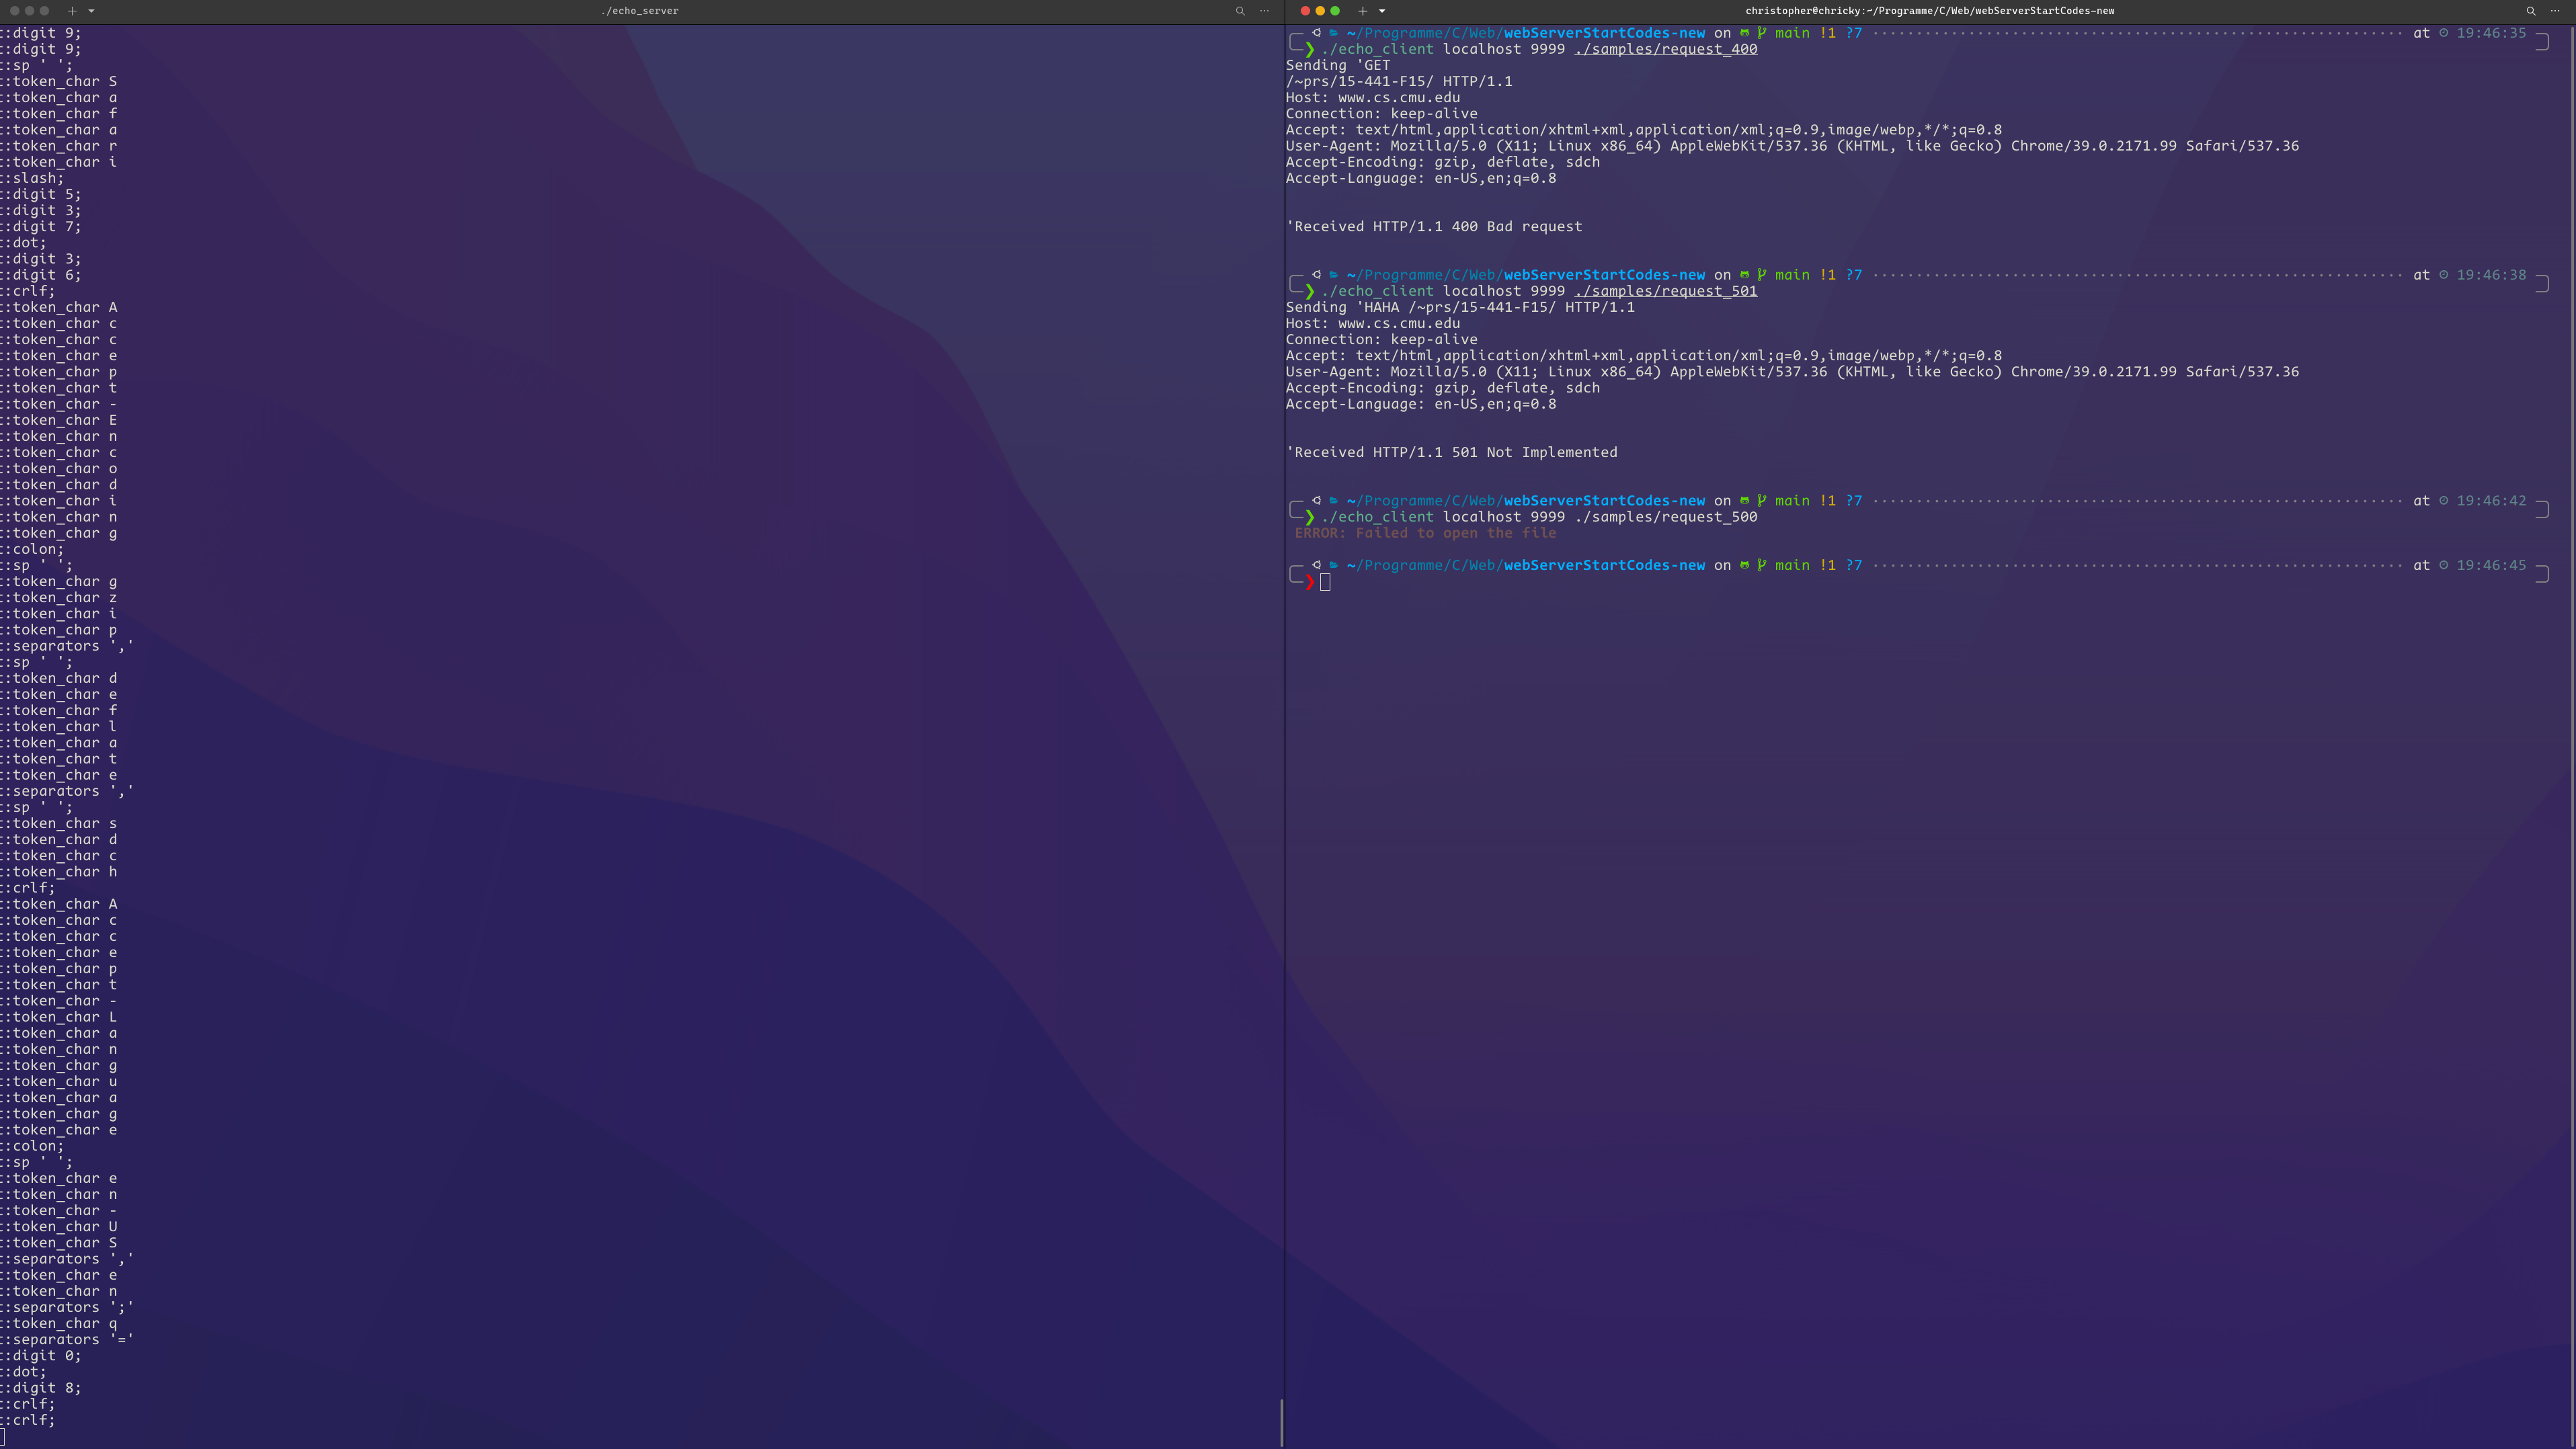
\includegraphics[width=2.5in]{400_501.png}}
    \caption{echo web server}\label{fig:echo web server}
    \vspace{-1em}
\end{figure}

\section{第二周——实现 HEAD、GET、POST 方法}

对于第二周的实验,我们使用了 API FOX 测试 GET, HEAD 以及 404 的返回(如图\ref{fig:apifox});使用浏览器测试服务器是否顺利返回文本、图片等(如图\ref{fig:web});使用liso\_client 测试新的缓冲区管理办法(如图\ref{fig:buffer})。均通过。

\begin{figure}[htbp!]
    \centering
    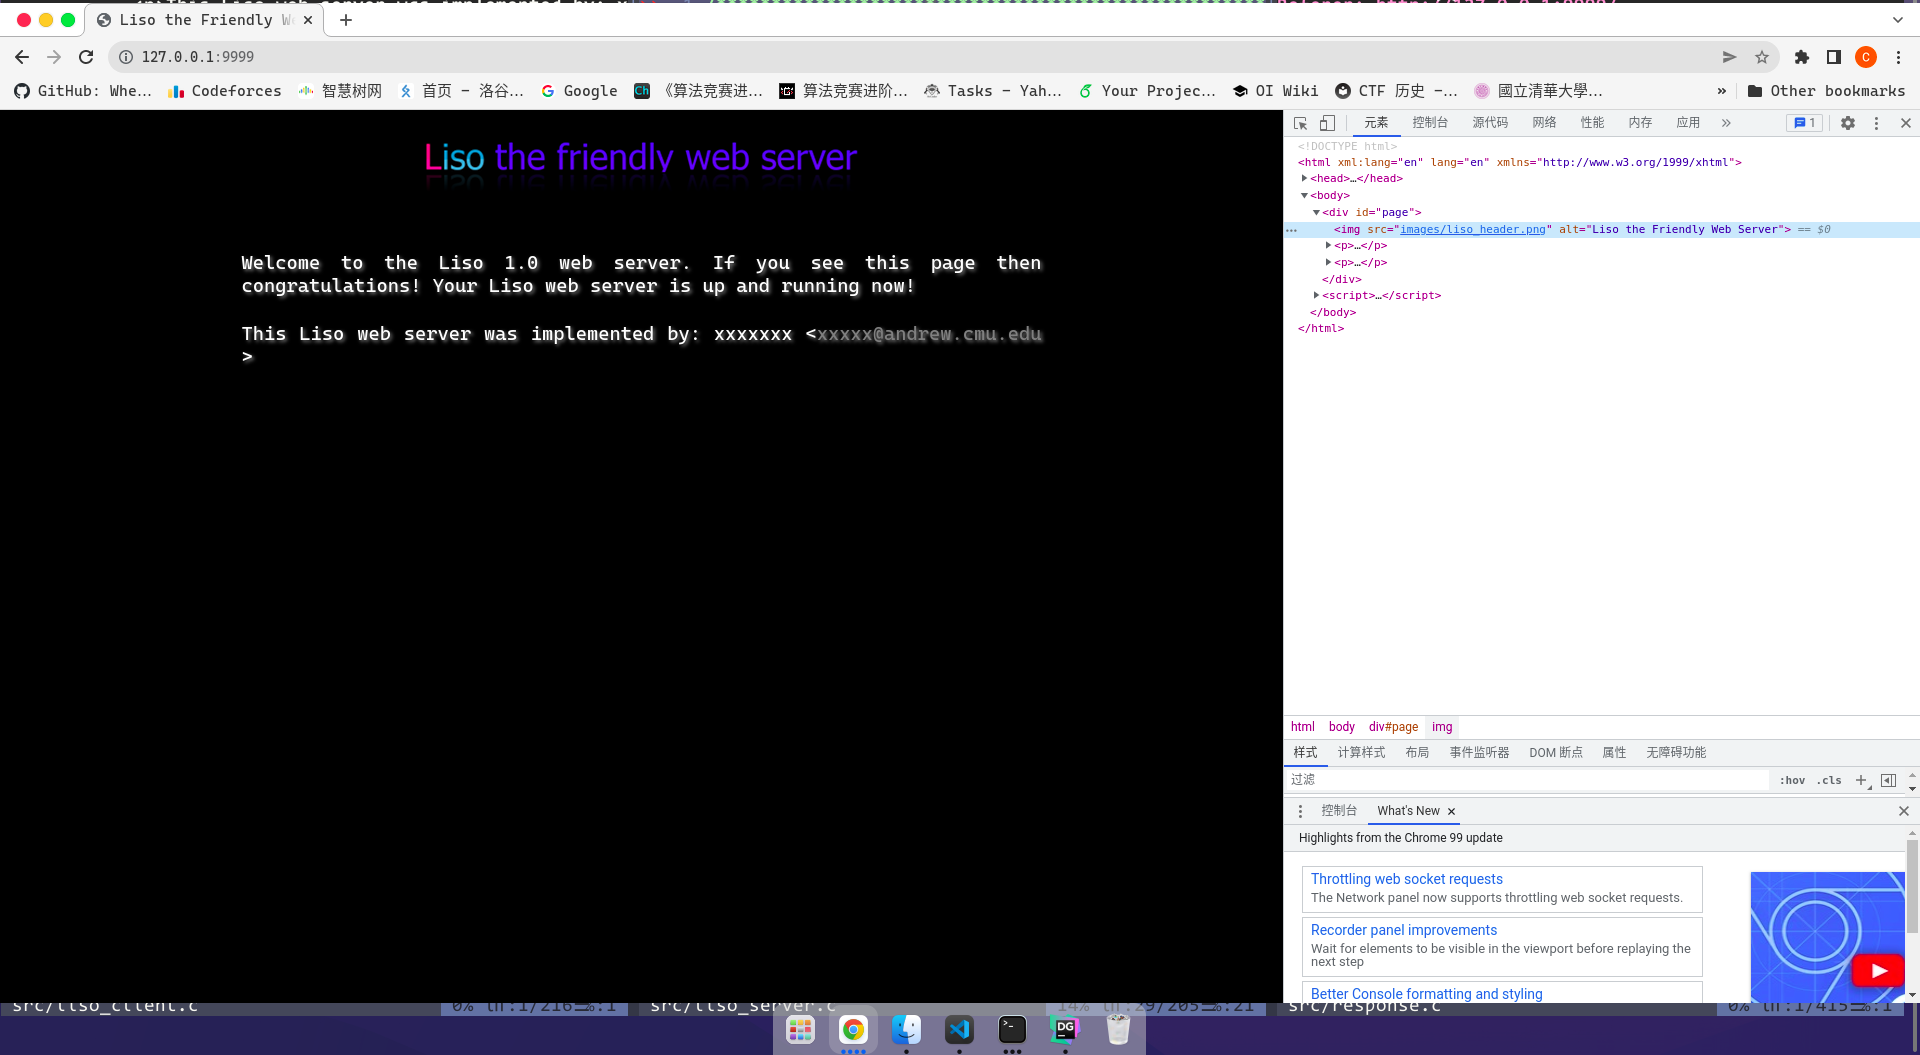
\includegraphics[width=5.5in]{liso_web.png}
    \caption{Liso Web Test}\label{fig:web}
\end{figure}

\subsection{结果分析}
在浏览器的测试中,发现和使用 liso\_client 测试不同,当出现有 404 的情况时,我们的 liso\_server 不会立刻进入下一轮监听,而是一直处于处理请求的情况。我们推测,是由于没实现 chunk 导致的。

\subsection{日志}
日志信息如图\ref{fig:logger} 所示。在日志信息里可以看到,我们的 recv 操作,每次最多接收 1025 字节的信息,单次可能不能完全接收一份报文的所有信息,但通过我们动态数组的管理,我们能够轻易完成 Pipeline 的测试。

\begin{figure}[htbp!]
    \centering
    \subfigure[Liso API FOX Test]{\label{fig:apifox}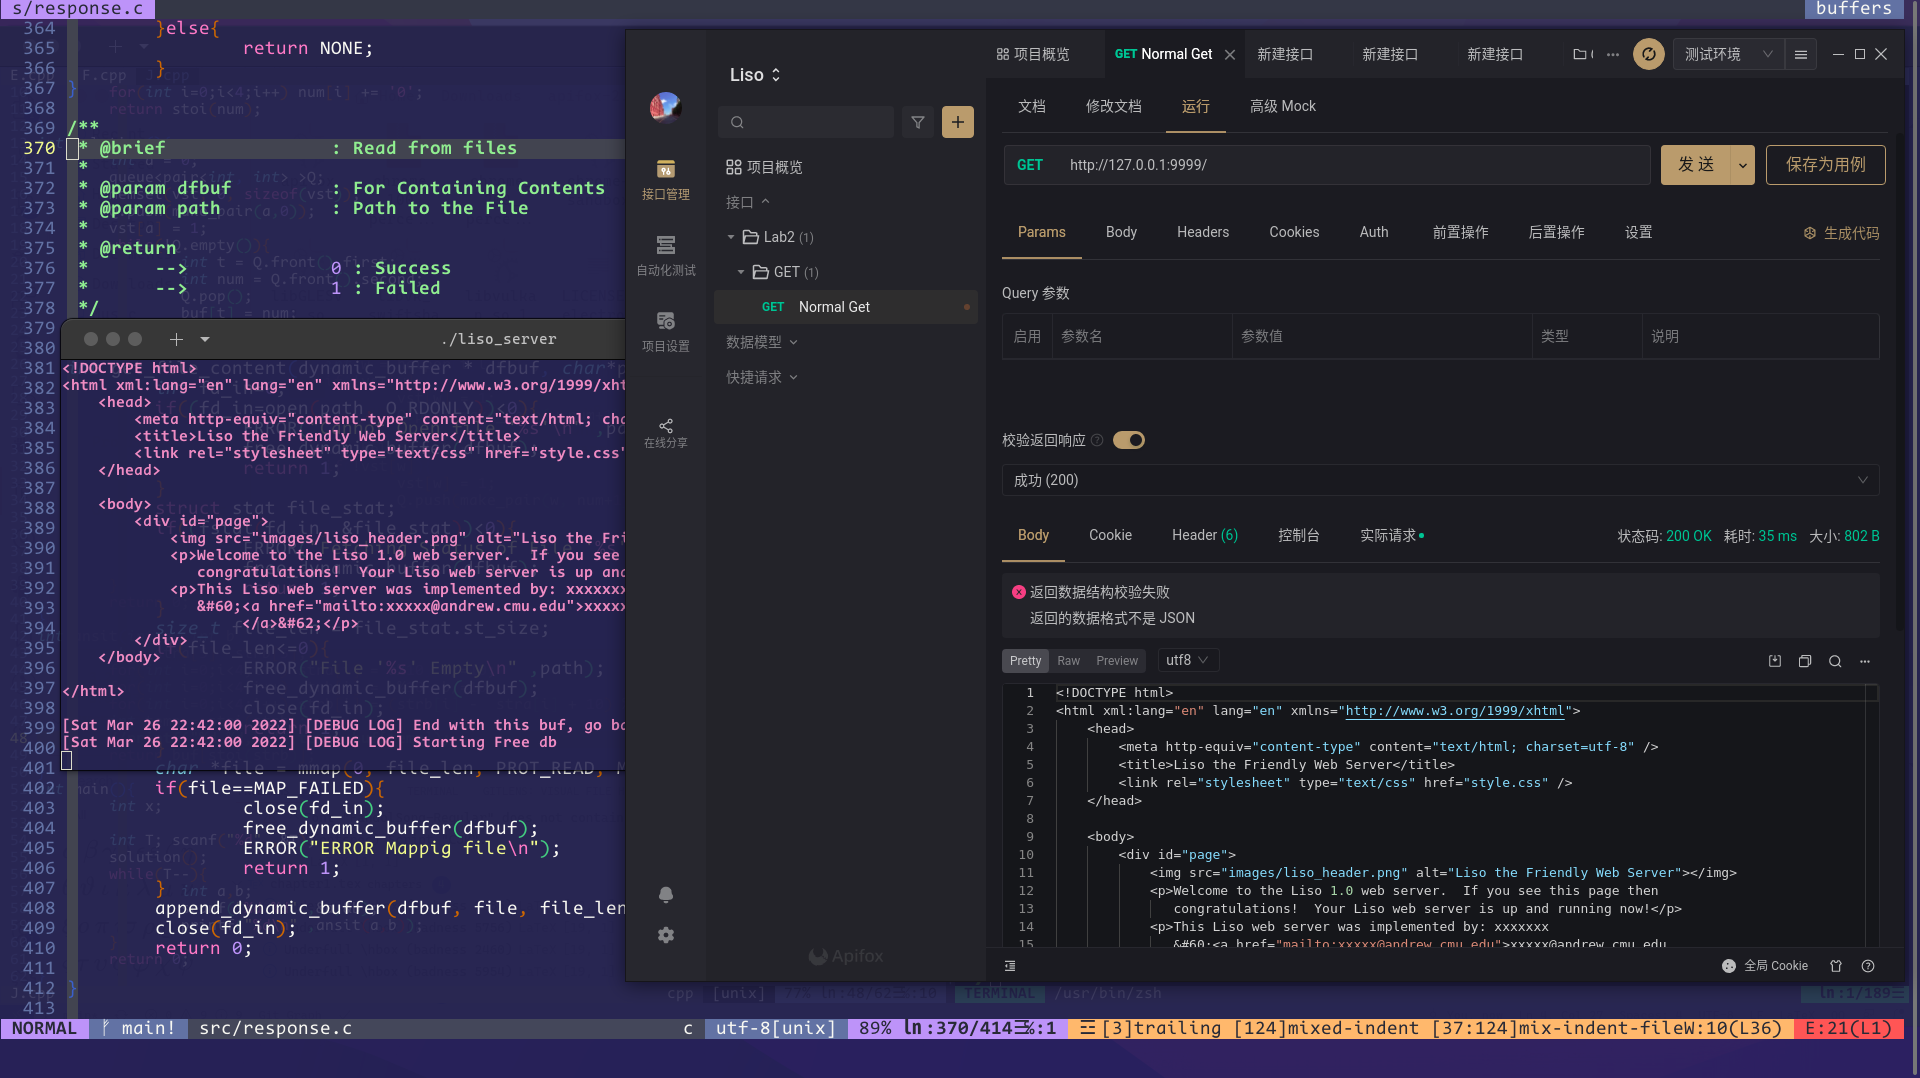
\includegraphics[width=2.75in]{APIFox_NormalGet.png}}
    \subfigure[Liso Test]{\label{fig:normal}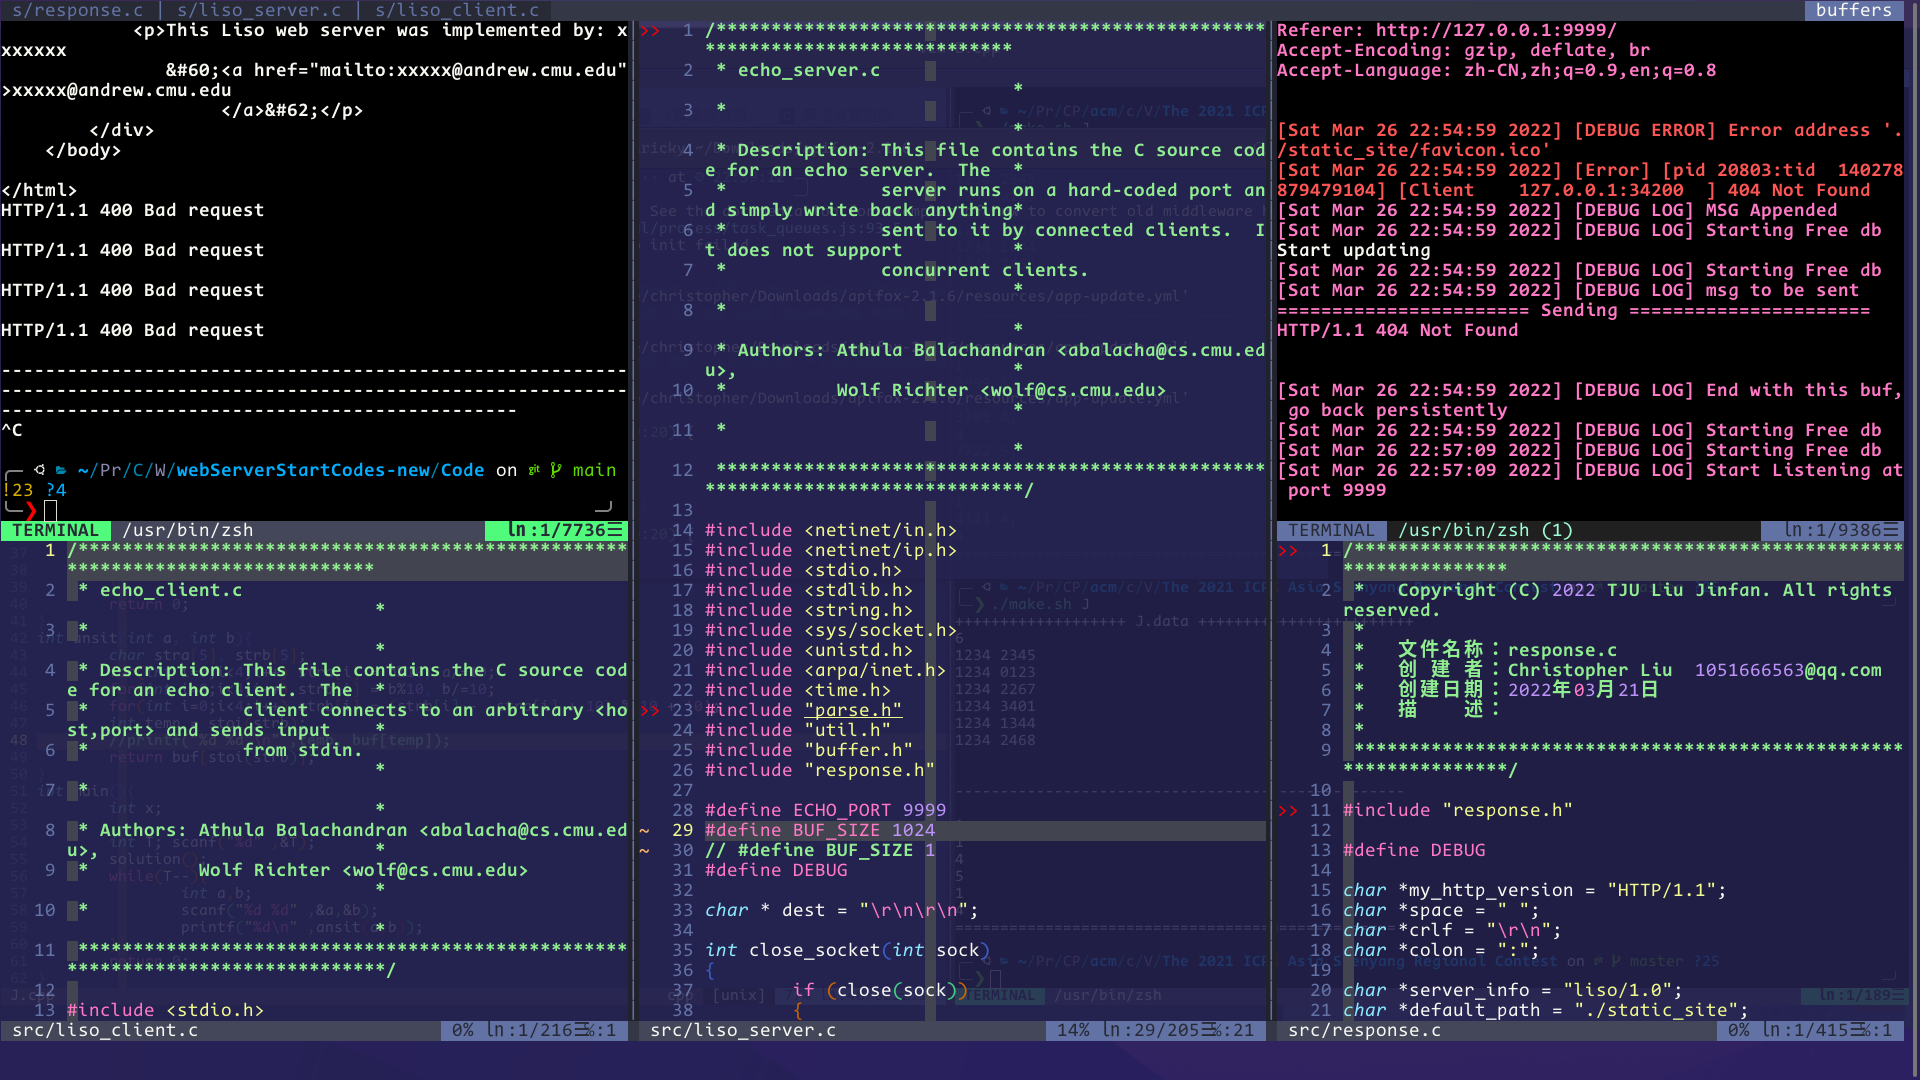
\includegraphics[width=2.75in]{liso_test.png}}
    \subfigure[部分 log 输出]{\label{fig:logger}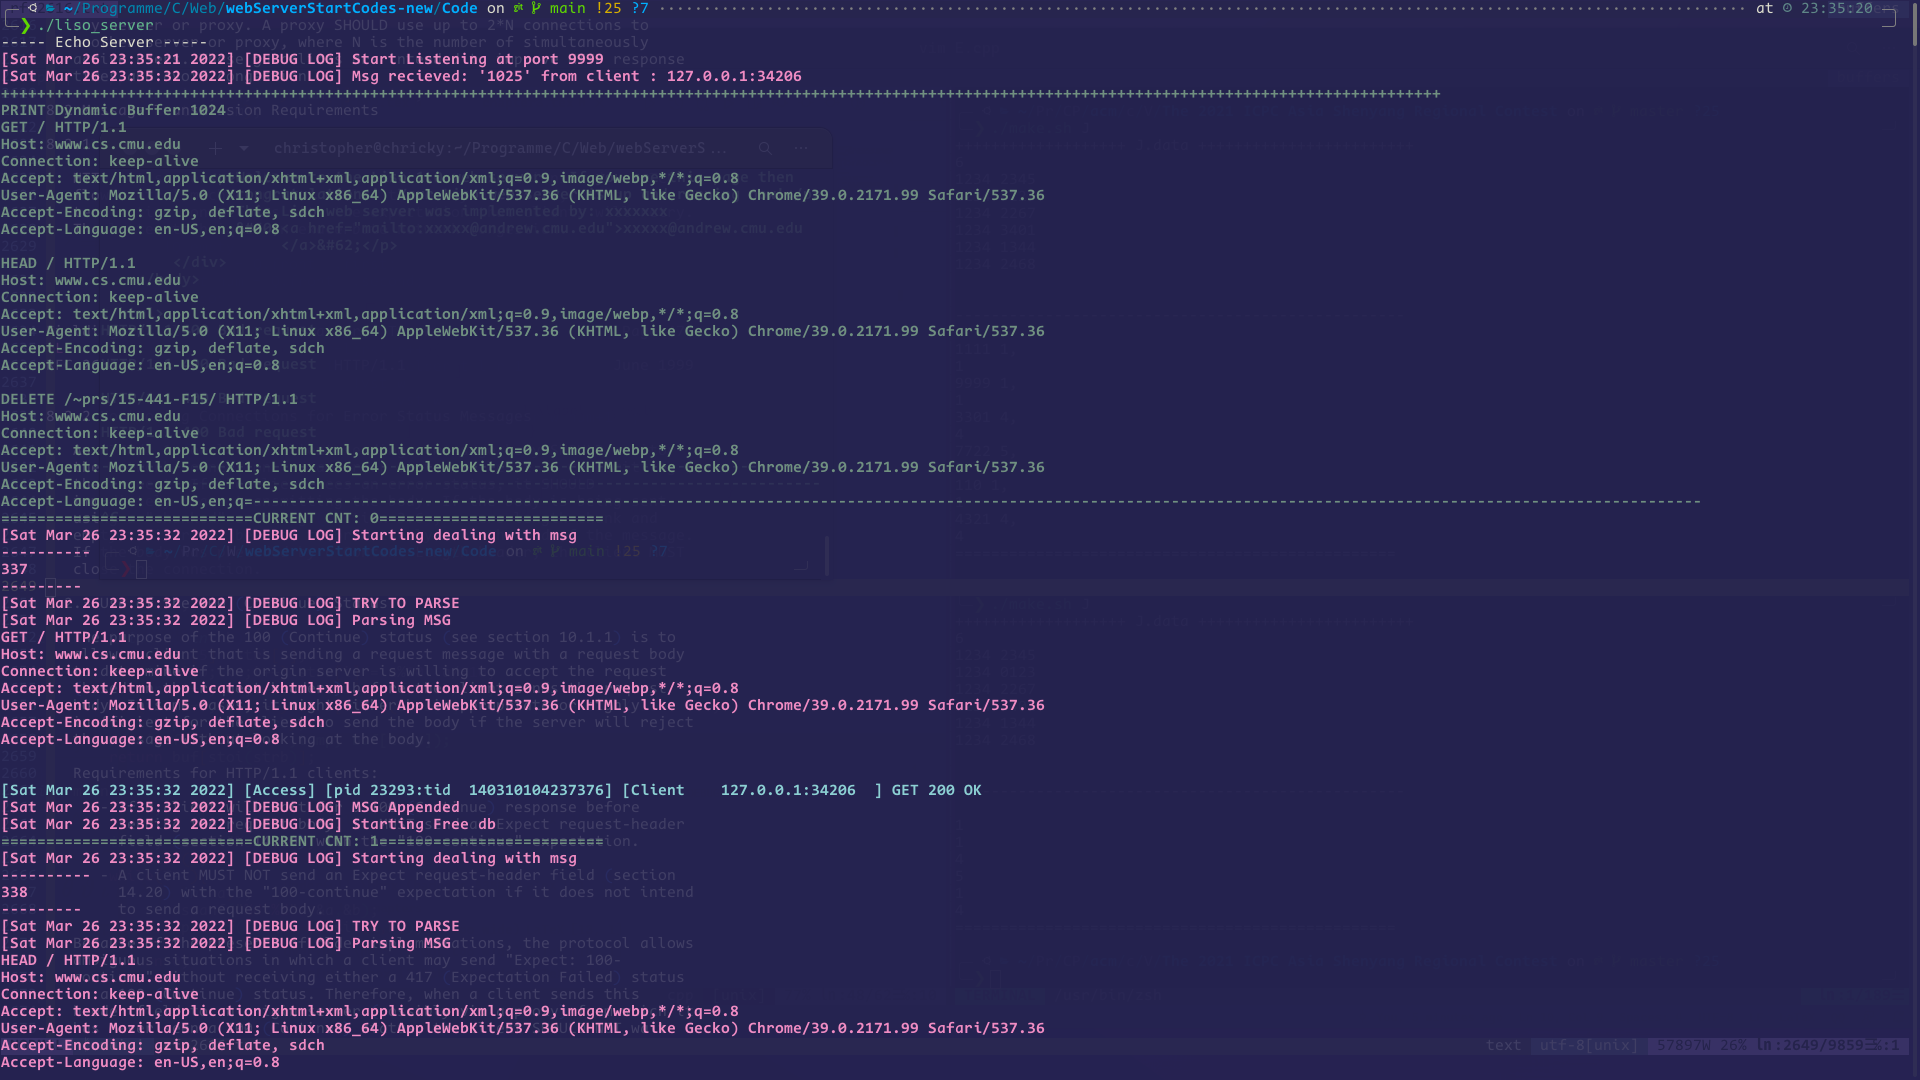
\includegraphics[width=5.5in]{lab2Logger.png}}
    \caption{测试结果展示}\label{fig:result}
\end{figure}


\section{第三周——实现HTTP的并发请求}


\subsection{pipelining 测试}

如图\ref{fig:pipelining},我们在request\_pipeline中客户端同一个TCP向服务器发送多个并发请求。我们根据服务器返回的实验结果来看(以最后几个为例)。第一个请求是GET方法,格式等也均是正确的,服务器也能正确解析返回给客户端消息;而第二个是HAHA方法,这个我们没有实现过,即返回“HTTP/1.1 501 Not Implemented\textbackslash r\textbackslash n\textbackslash r\textbackslash n”。

而第三个是/~prs/15-441-F15/HTTP/1.1,存在格式错误,因此服务器返回“HTTP/1.1 400 Bad request\textbackslash r\textbackslash n\textbackslash r\textbackslash n”。服务器能够识别这个错误请求并拒绝了这个请求,也能继续识别并发的下一条请求。下一条请求HTTP/1.30也存在格式错误,同样,服务器能够在拒绝上一条错误请求之后解析这条这条请求。根据结果来看,我们的实现是正确的。对于这个结果,我们也容易从代码分析出来这是正确的。我们引入了strstr(str,dest)函数,我们就能找到”\textbackslash r\textbackslash n\textbackslash r\textbackslash n”的位置。找到了”\textbackslash r\textbackslash n\textbackslash r\textbackslash n”的位置之后,也很容易找到单个报文,我们之前已经实现了正确解析单个报文。所以我们处理出来了单个报文之后也就能正确处理这些并发的请求了。

\begin{figure}[htbp!]
    \centering 
    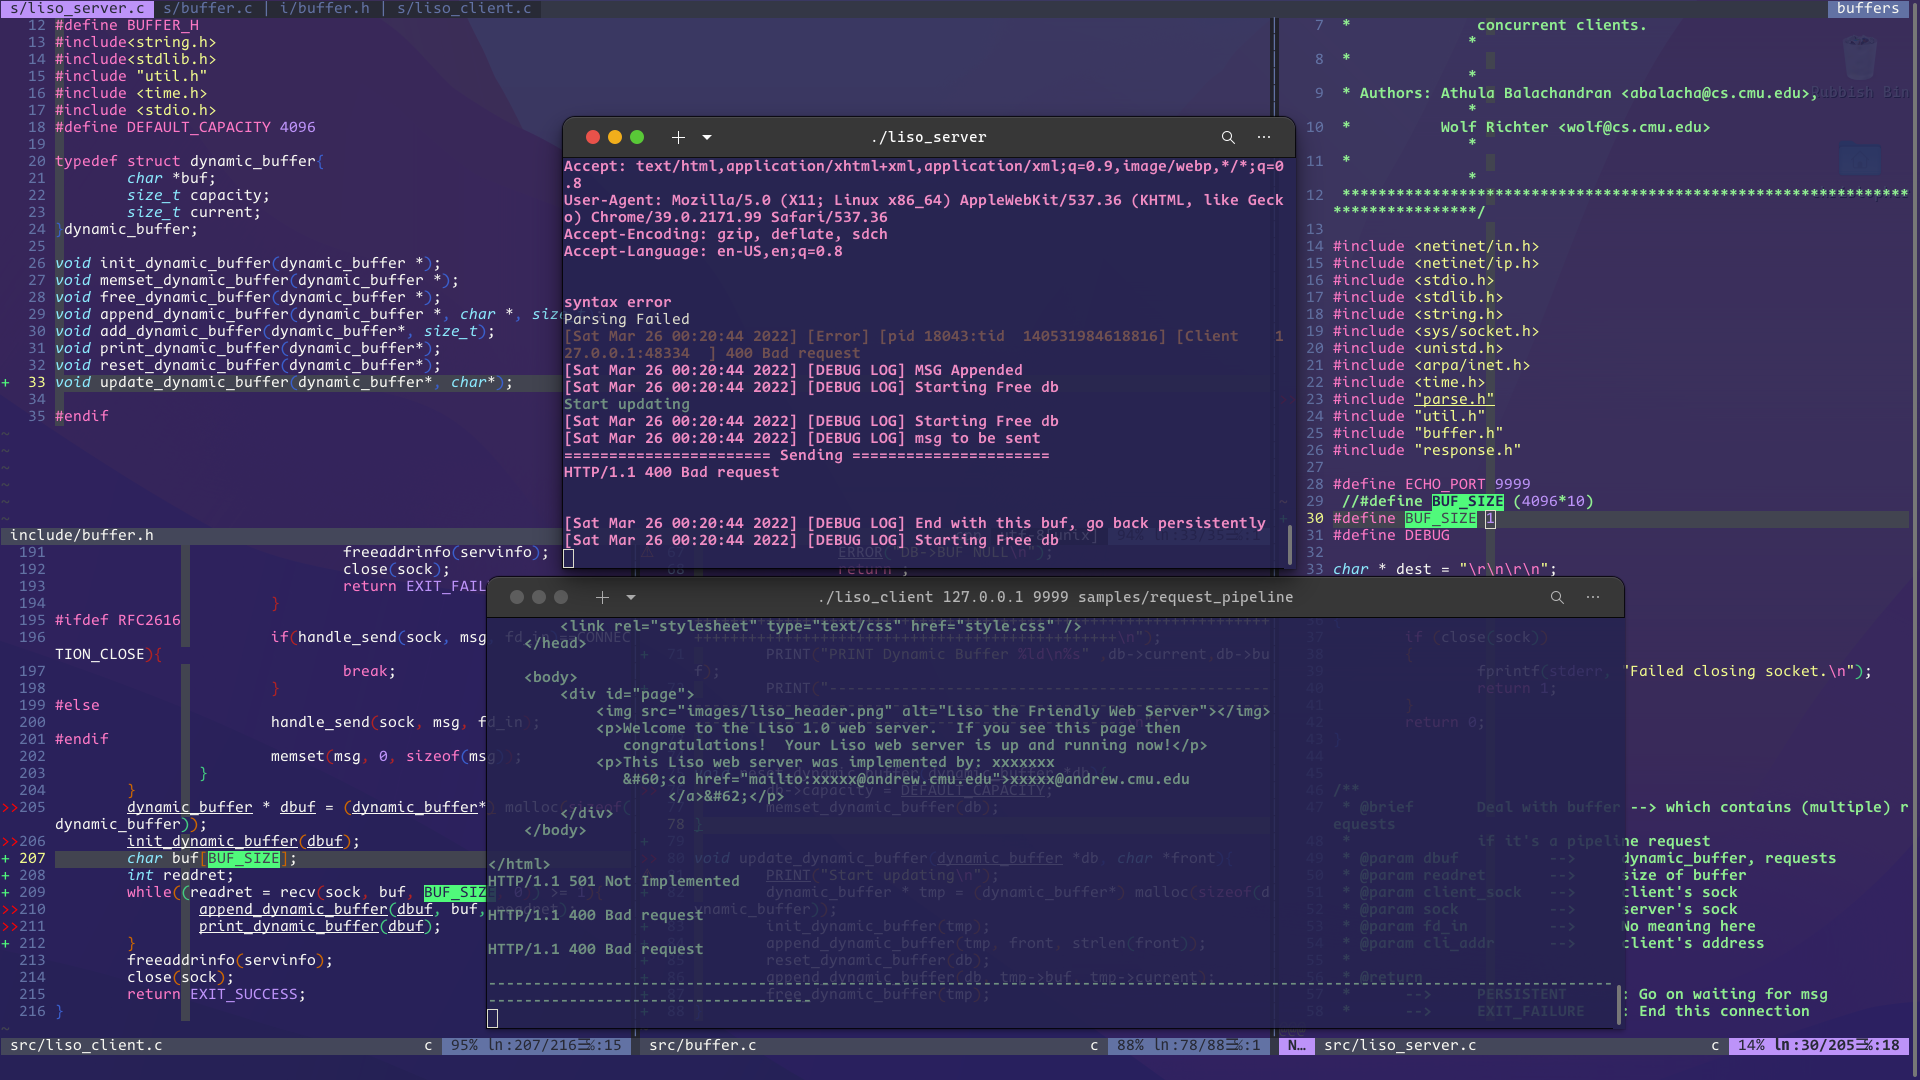
\includegraphics[width=5.5in]{BUF=1.png}
    \caption{pipelining test}
    \label{fig:pipelining}
\end{figure}


\section{第四周——实现多个客户端的并发处理}

\subsection{手工测试}
我们将 liso\_client 设置为忙等待,及其不会自动关闭 socket 并退出,而是占用着服务器的资源等待着。如图\ref{fig:lab4test1},我们同时开启了 4 个陷入忙等待的客户端对服务器发出请求,服务器仍然能正常处理发出 pipeline 请求的客户端。


\begin{figure}[htbp!]
    \centering 
    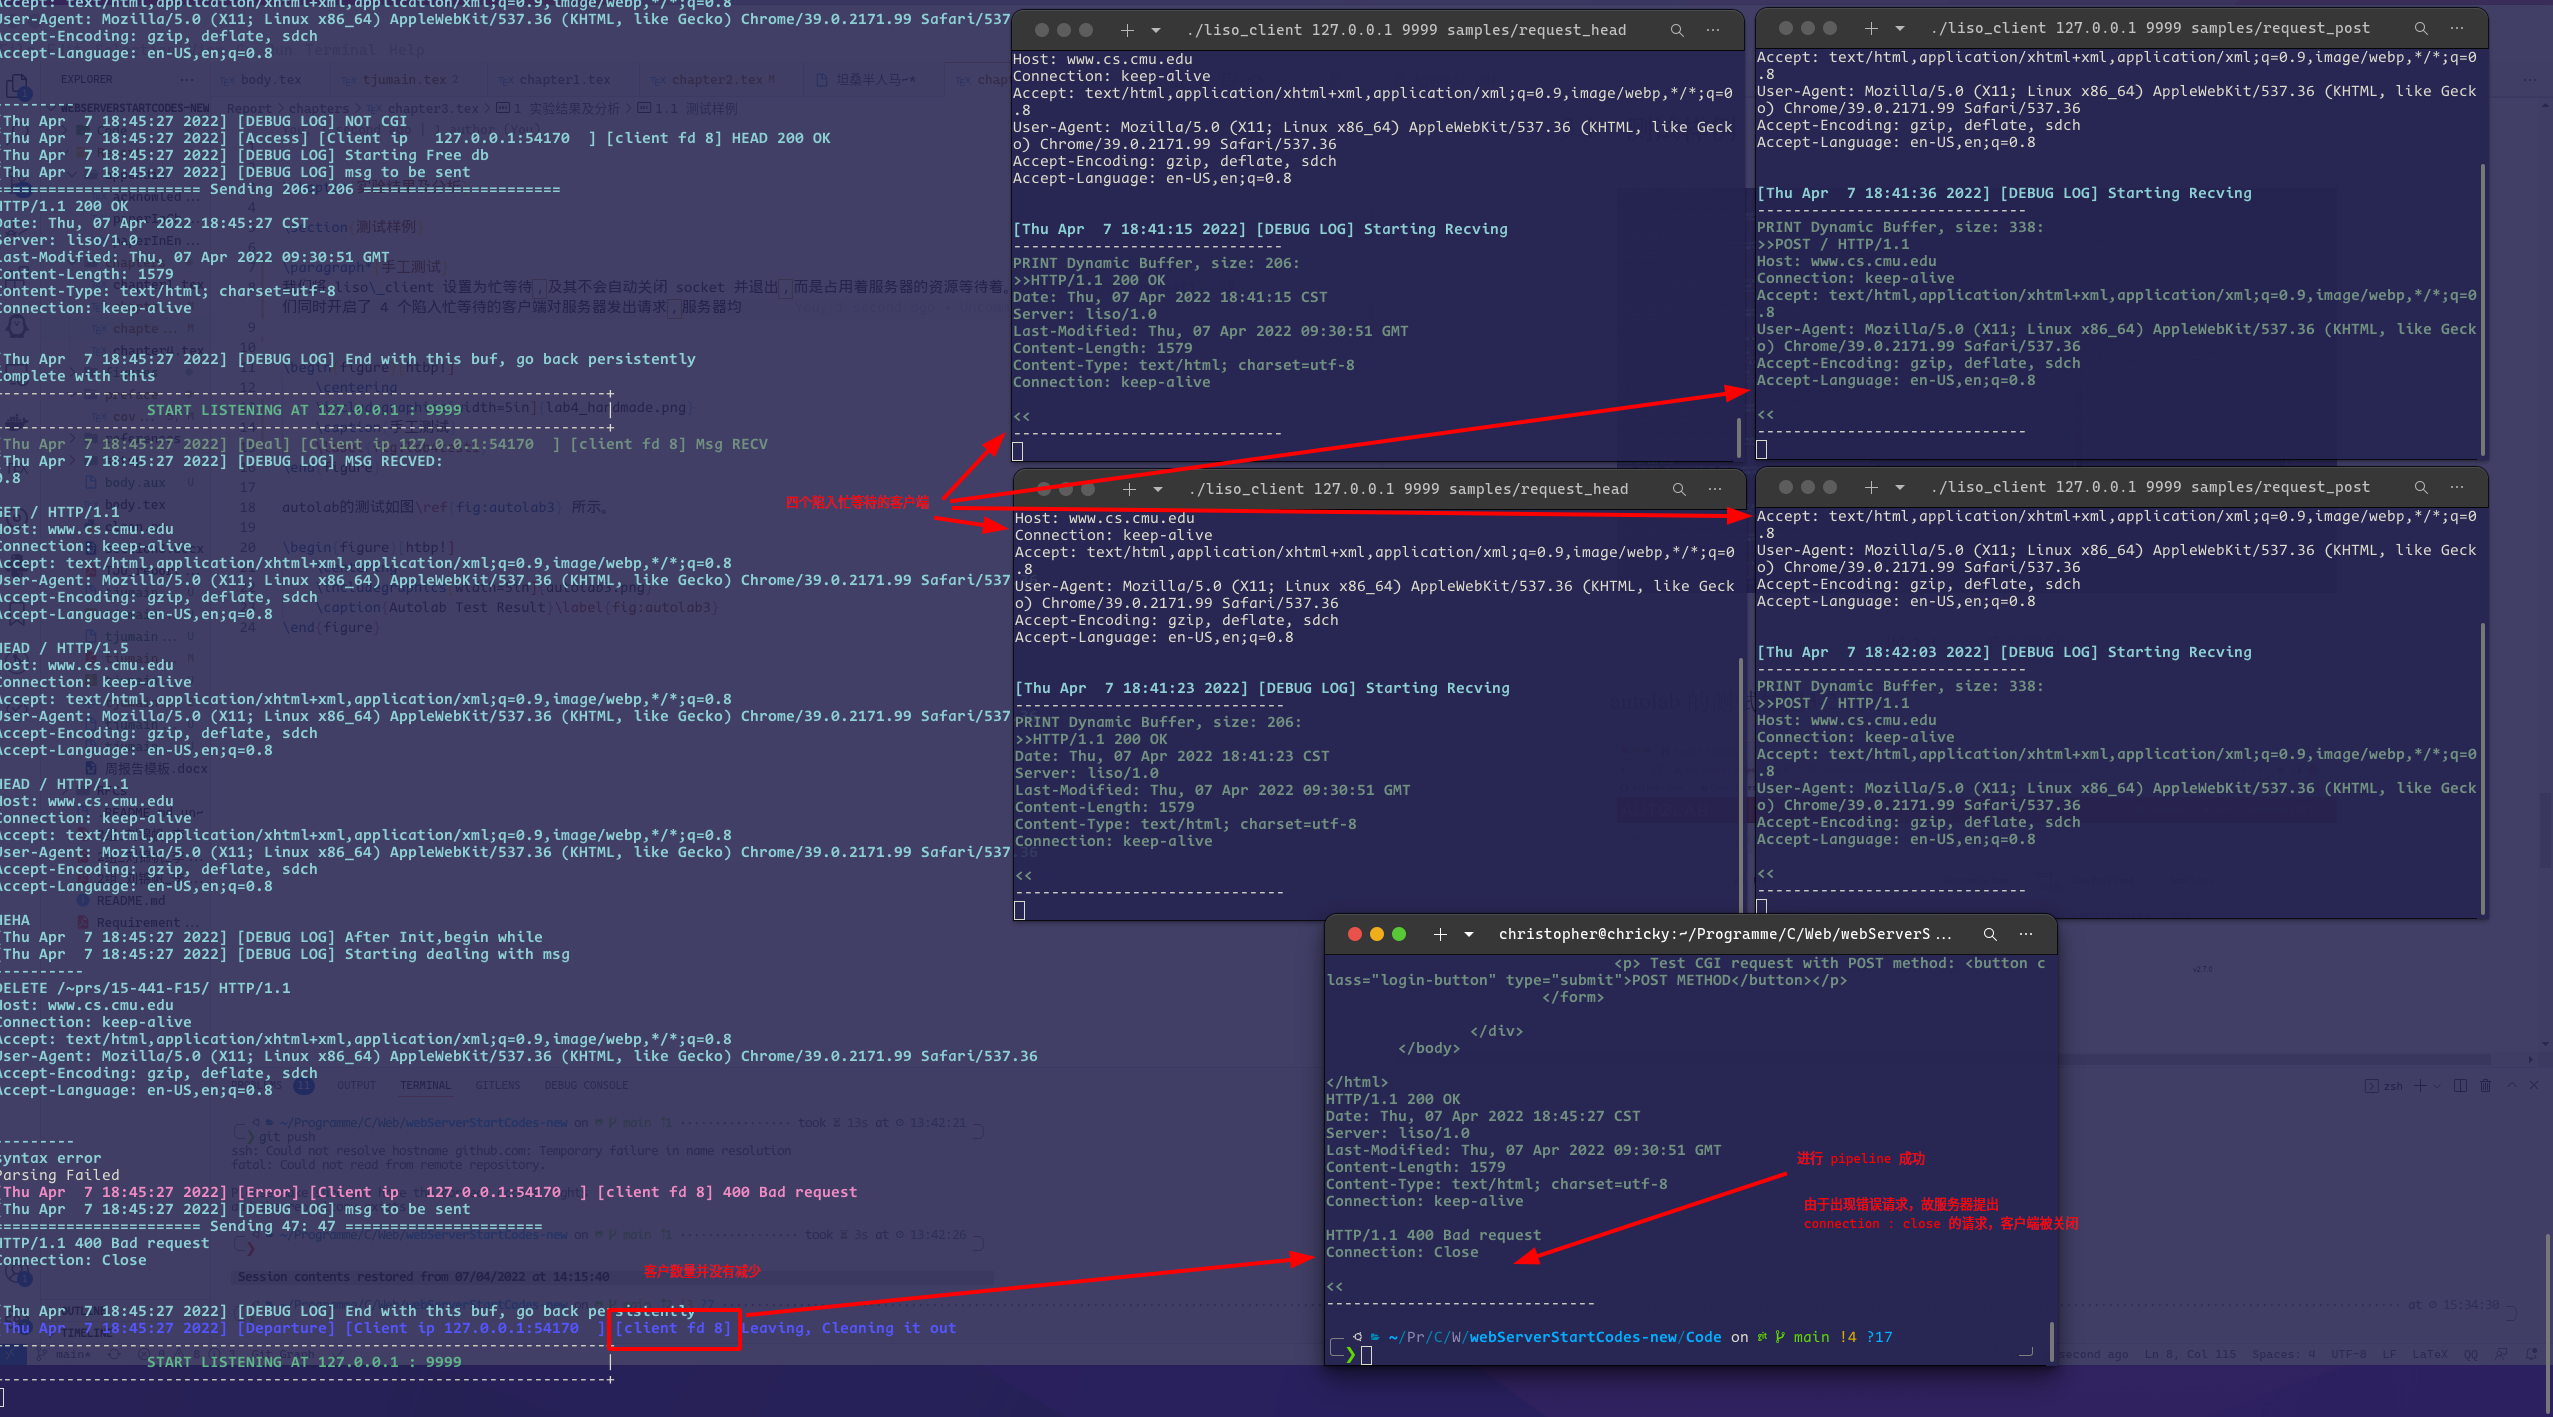
\includegraphics[width=5.6in]{lab4_handmade.png}
    \caption{手工测试}
    \label{fig:lab4test1}
\end{figure}

\subsection{Apache 测试} 

第三周的 liso\_server 由于没有进行并发优化。在测试时由于会一直等待客户端提出退出申请,在测试时会出现 Apache Bench 忙等待。我们分别进行了并发压力测试以及多请求压力测试。测试截图统一放在附录中。

\paragraph*{并发压力测试} 控制总请求数不变的情况下,我们分别进行了并发数量为 10、100 以及 1000 的测试,结果如图所示。如表\ref{tab:parallel} 所示,总请求数量不变情况下,随着并发等级的提高,单个请求的平均反应时间并没有太大的变化。所以可以认为我们的方案是能够解决高并发问题的。

\begin{table}[htbp!]
    \centering
    \begin{tabular}{llll}\hline
      & 并发等级 & 总请求数量 & TPR(ms)   \\\hline
    1 & 10   & 1000  & 0.378 \\
    2 & 100  & 1000  & 0.390 \\
    3 & 1000 & 1000  & 0.429\\
    \hline
    \end{tabular}
    \caption{并发压力测试结果}\label{tab:parallel}
\end{table}

\paragraph*{多请求压力测试} 通过控制并发等级为10不变,改变总请求数量,我们得到了多请求压力测试的结果,如表\ref{tab:multiple}所示。可以轻易看出,在并发等级一定的情况下,总请求数量在100,000量级及以下时,单个请求的平均反应时间都能在正常的范围中。但当请求量达到1,000,000 数量级时,单个请求的平均相应时间则会增加很多,推测是因为请求数量太多,导致频繁接受、删除用户,进而导致反应时间增加。

\begin{table}[htbp!]
    \centering
    \begin{tabular}{llll}\hline
      & 并发等级 & 总请求数量 & TPR(ms)   \\\hline
    1 & 10      & 100       & 0.395 \\
    2 & 10      & 1000      & 0.378 \\
    3 & 10      & 10000     & 0.364\\
    4 & 10      & 100000    & 0.445\\
    5 & 10      & 1000000   & 0.781\\
    \hline
    \end{tabular}
    \caption{多请求压力测试}\label{tab:multiple}
\end{table}

\section{选做——CGI}

